\documentclass[a0,portrait]{a0poster}

\usepackage{graphicx}
\usepackage{amsmath}
\usepackage{amssymb}
\usepackage{multirow}
\usepackage{multicol} % This is so we can have multiple columns of text side-by-side
\columnsep=100pt % This is the amount of white space between the columns in the poster
\columnseprule=3pt % This is the thickness of the black line between the columns in the poster
% \usepackage{hyperref}


\usepackage[svgnames]{xcolor} % Specify colors by their 'svgnames', for a full list of all colors available see here: http://www.latextemplates.com/svgnames-colors

% \usepackage{times} % Use the times font
\usepackage{palatino} % Uncomment to use the Palatino font

\usepackage{graphicx} % Required for including images
\graphicspath{{figures/}} % Location of the graphics files
\usepackage{booktabs} % Top and bottom rules for table
\usepackage[font=small,labelfont=bf]{caption} % Required for specifying captions to tables and figures
\usepackage{amsfonts, amsmath, amsthm, amssymb} % For math fonts, symbols and environments
\usepackage{wrapfig} % Allows wrapping text around tables and figures

\usepackage{amsthm}

\usepackage[utf8]{inputenc}
\usepackage{algorithm}
\usepackage[noend]{algpseudocode}



\newtheorem{lemma}{Lemma}
\newtheorem{thm}{Theorem}
\newtheorem{prop}{Proposition}


\begin{document}

%----------------------------------------------------------------------------------------
% POSTER HEADER
%----------------------------------------------------------------------------------------

% The header is divided into two boxes:
% The first is 75% wide and houses the title, subtitle, names, university/organization and contact information
% The second is 25% wide and houses a logo for your university/organization or a photo of you
% The widths of these boxes can be easily edited to accommodate your content as you see fit

\begin{minipage}[b]{0.75\linewidth}
\VeryHuge \color{NavyBlue} \textbf{Gradient Flow Optimizers} \color{Black}\\ % Title
\huge \textbf{Raghav K Singhal}\\[0.5cm] % Author(s)
\huge New York University\\[0.4cm] % University/organization
\end{minipage}

\vspace{1cm} % A bit of extra whitespace between the header and poster content
%---------------------------------------------------------------------------------------
\begin{multicols}{3} % This is how many columns your poster will be broken into, a portrait poster is generally split into 2 columns

%----------------------------------------------------------------------------------------
% ABSTRACT
%----------------------------------------------------------------------------------------
\color{Navy} % Navy color for the abstract
\begin{abstract}
In recent years there has been a great interest in using Differential Equations to model and understand the behaviour of Optimization Algorithms, as a closer look at Gradient Descent Algorithm shows that it is an Euler-Approximation to a certain Ordinary Differential Equation. Our work here shows that we can take the Differential Equation approach further, building new classes of optimizers based on integration techniques for Differential Equations.
\end{abstract}
%----------------------------------------------------------------------------------------
% INTRODUCTION
%----------------------------------------------------------------------------------------

\color{Black} % SaddleBrown color for the introduction
\section*{Gradient Flow Equation}
Gradient Descent has a very simple interpretation as a First-Order Integration scheme for the gradient flow equation,
\begin{align*}\vspace{1cm}
\dot{x}_t = -\nabla f(x_t)
\end{align*}
\color{Black} % SaddleBrown color for the introduction
And then based on the following result for strongly convex functions we explore using other integration schemes for the optimization task,

\begin{prop}
Let $f \in \mathcal{S}_{\mu, \beta}^{2,1}$, and suppose $x^*$ is the global minimum, then the solution trajectory to the gradient flow equation satisfies the following:
\begin{align*}\vspace{1cm}
f(x_t) - f(x^*) &\leq e^{-2 \mu t} \big( f(x_0) - f(x^*) \big) \\
\| x_t - x^* \|^2 &\leq e^{-2 \mu t} \| x_0 - x^* \|^2
\end{align*}
\end{prop}

And also a similar but weaker result holds for general $f$, as the set of critical points of $f$ are in the $\omega$-limit set for $\dot{x}_t = -\nabla f(x_t)$. Where the $\omega$-limit set is defined as:
\begin{align*}\vspace{1cm}
\omega(x_0) = \{x: \forall T &\text{ and } \epsilon > 0, \exists t>T, |\phi (x_t, x_0) - x|<\epsilon \}
\end{align*}\vspace{1cm}
where $\phi(x_t,x_0)$ is the flow of the gradient flow equation and $x_0$ is the initial condition.
% \begin{itemize}
% \item Geothermal exploration program started in 1967 by National Oil Comapny SONATRACH.
% \item From 1983 onwards the geothermal research has been continued by the Renewable Energies Center of Algeria (CDER).
% \end{itemize}
%----------------------------------------------------------------------------------------
% GEOLOGY
%----------------------------------------------------------------------------------------

\color{Black} % DarkSlateGray color for the rest of the content

\section*{Runge-Kutta Methods}
Runge-Kutta Methods refer to a family of Integration Schemes consisting of explicit and implicit methods. There are several advantages to using Runge-Kutta methods, which can be
found in the Numerical Analysis Literature.
%----------------------------------------------------------------------------------------
% GEOTHERMAL DATA
%----------------------------------------------------------------------------------------
\section*{}
\subsection*{Runge-Kutta 4th Order }
This is the most well known of the Runge-Kutta Families, commonly known as RK4. This Scheme is given by:

\begin{align*}
k_1 &= \nabla f(x_k) \\
k_2 &= \nabla f(x_k - \frac{\alpha}{2} \nabla f(x_k)) \\
k_3 &= \nabla f(x_k - \frac{\alpha}{2}\nabla k_2) \\
k_4 &= \nabla f(x_k - \alpha k_3)      \\
x_{k+1} &= x_k + \frac{\alpha}{6}(k_1 + 2k_2 + 2k_3 + k_4)
\end{align*}

% \begin{center}\vspace{1cm}
% \includegraphics[width=1.0\linewidth]{Fig2}
% \captionof{figure}{\color{Green} (A) Temp. vs. depth for different regions (Takherist and Lesquer, 1989). (B) Heat flow map of Algeria (Takherist and Lesquer, 1989). Unit: mW/m$^2$. 230 oil wells are presented, with depths ranging from 500 to 5500 m.}
% \end{center}\vspace{1cm}

%------------------------------------------------

\subsection*{Runge-Kutta 2nd order - Ralston Method}

\begin{align*}
k_1 &= \nabla f(x_k) \\
k_2 &= \nabla f(x_k - \frac{2\alpha}{3} \nabla f(x_k)) \\
x_{k+1} &= x_k + \frac{\alpha}{4}(k_1 + 3k_2)
\end{align*}

\subsection*{Runge-Kutta 2nd order - Heun's Method}

\begin{align*}
k_1 &= \nabla f(x_k) \\
k_2 &= \nabla f(x_k - \alpha \nabla f(x_k)) \\
x_{k+1} &= x_k + \frac{\alpha}{2}(k_1 + k_2)
\end{align*}

\subsection*{Experiments}
\begin{center}
  \begin{tabular}{ | l | c | r| }
    \hline
    Model & RK2-Test Accuracy & RK2-Test Loss \\ \hline
    WideResNet & 93.07\% & 0.286  \\ \hline
    ResNet18 & 92.5\% & 0.212 \\ \hline
    Logistic Regression & 92.14\% & 0.0015  \\ \hline
    Lasso & 92.65\% & 0.0021 \\ \hline
    \hline
  \end{tabular}
\end{center}

\begin{center}
  \begin{tabular}{ | l | c | r| }
    \hline
    Model & SGD-Test Accuracy & SGD-Test Loss \\ \hline
    WideResNet & 92.95\% & 0.249 \\ \hline
    ResNet18  & 89.27\% & 0.1914 \\ \hline
    Logistic Regression & 91.95\% & 0.00101 \\ \hline
    Lasso & 92.52\% & 0.00210  \\ \hline
    \hline
  \end{tabular}
\end{center}

\subsection*{Neural Networks}
We do experiments with three main models:
\begin{itemize}
\item Resnet18 on CIAFR10
\item WideResnet on CIAFR10
\item Logistic Regression with Regularization on MNIST
\end{itemize}

\subsection*{ResNet18}
\begin{center}\vspace{1cm}
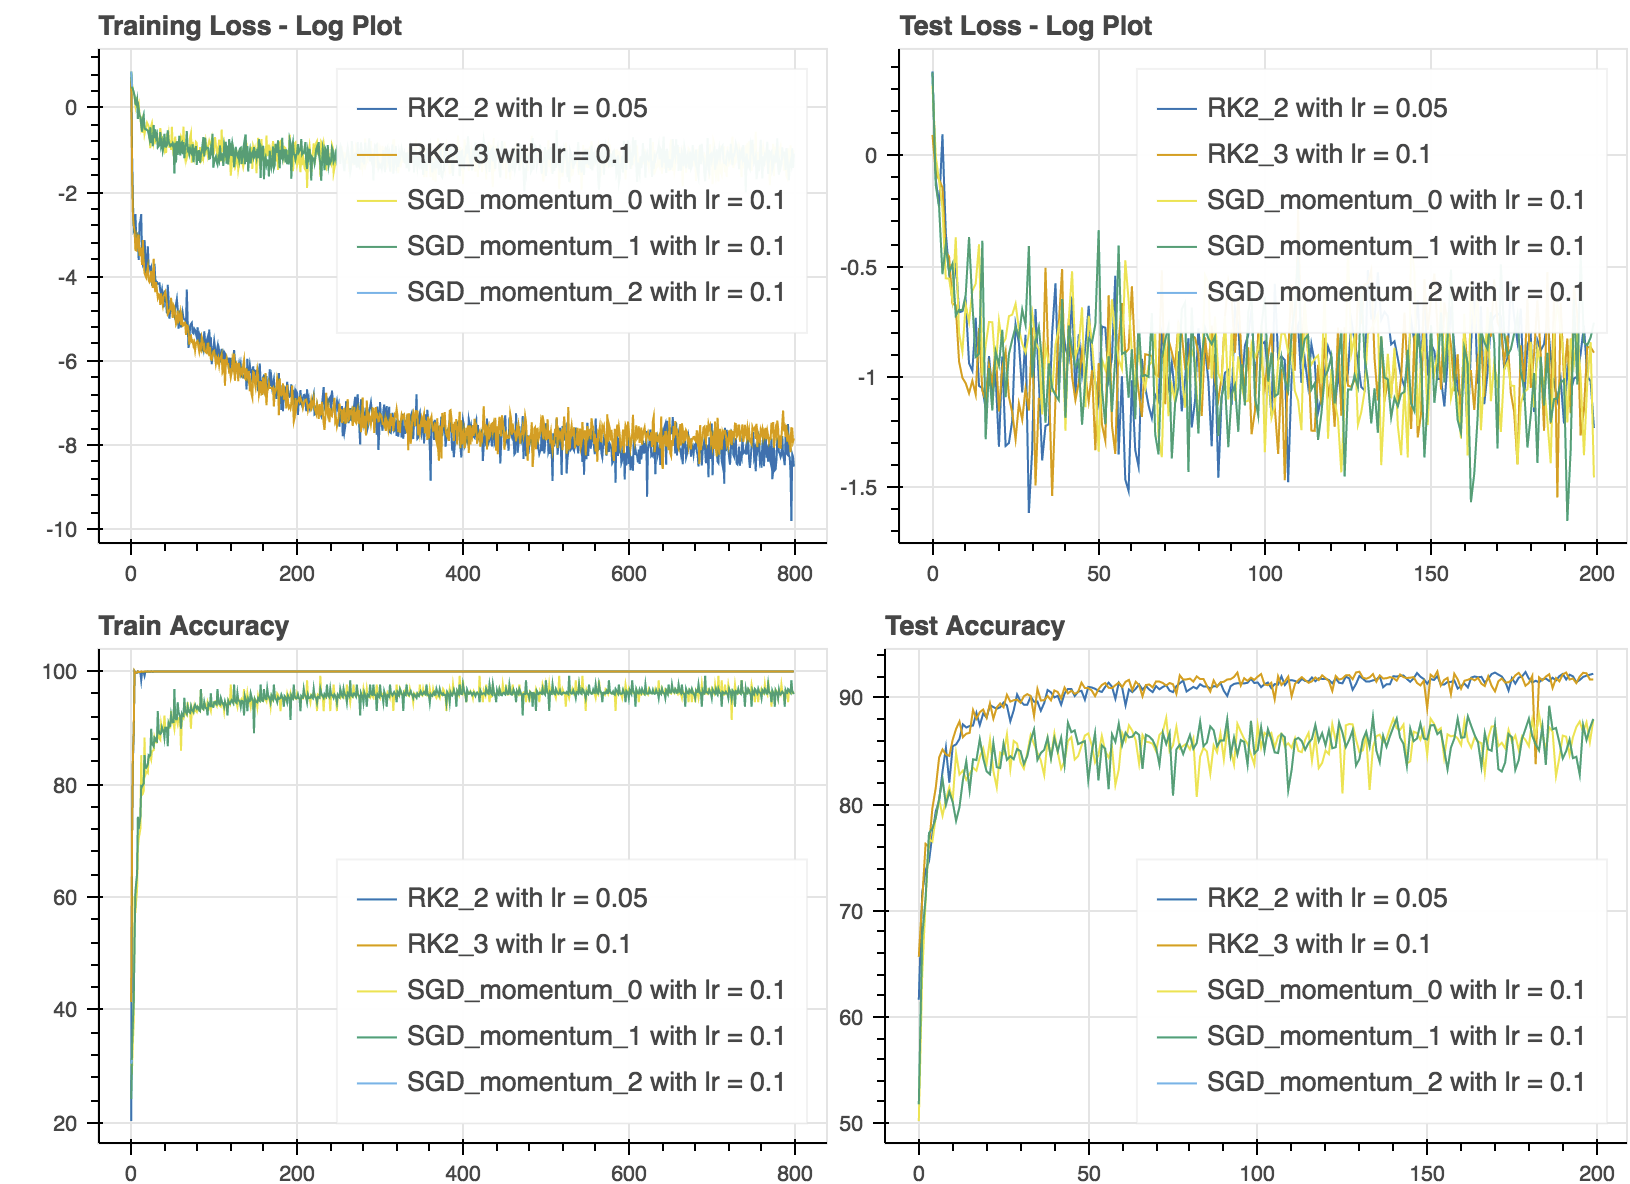
\includegraphics[width=0.8\linewidth]{../plots/inf_plots/resnet_sgd_rk2.png}
\end{center}%\vspace{1cm}

\subsection*{WideResNet}
\begin{center}\vspace{1cm}
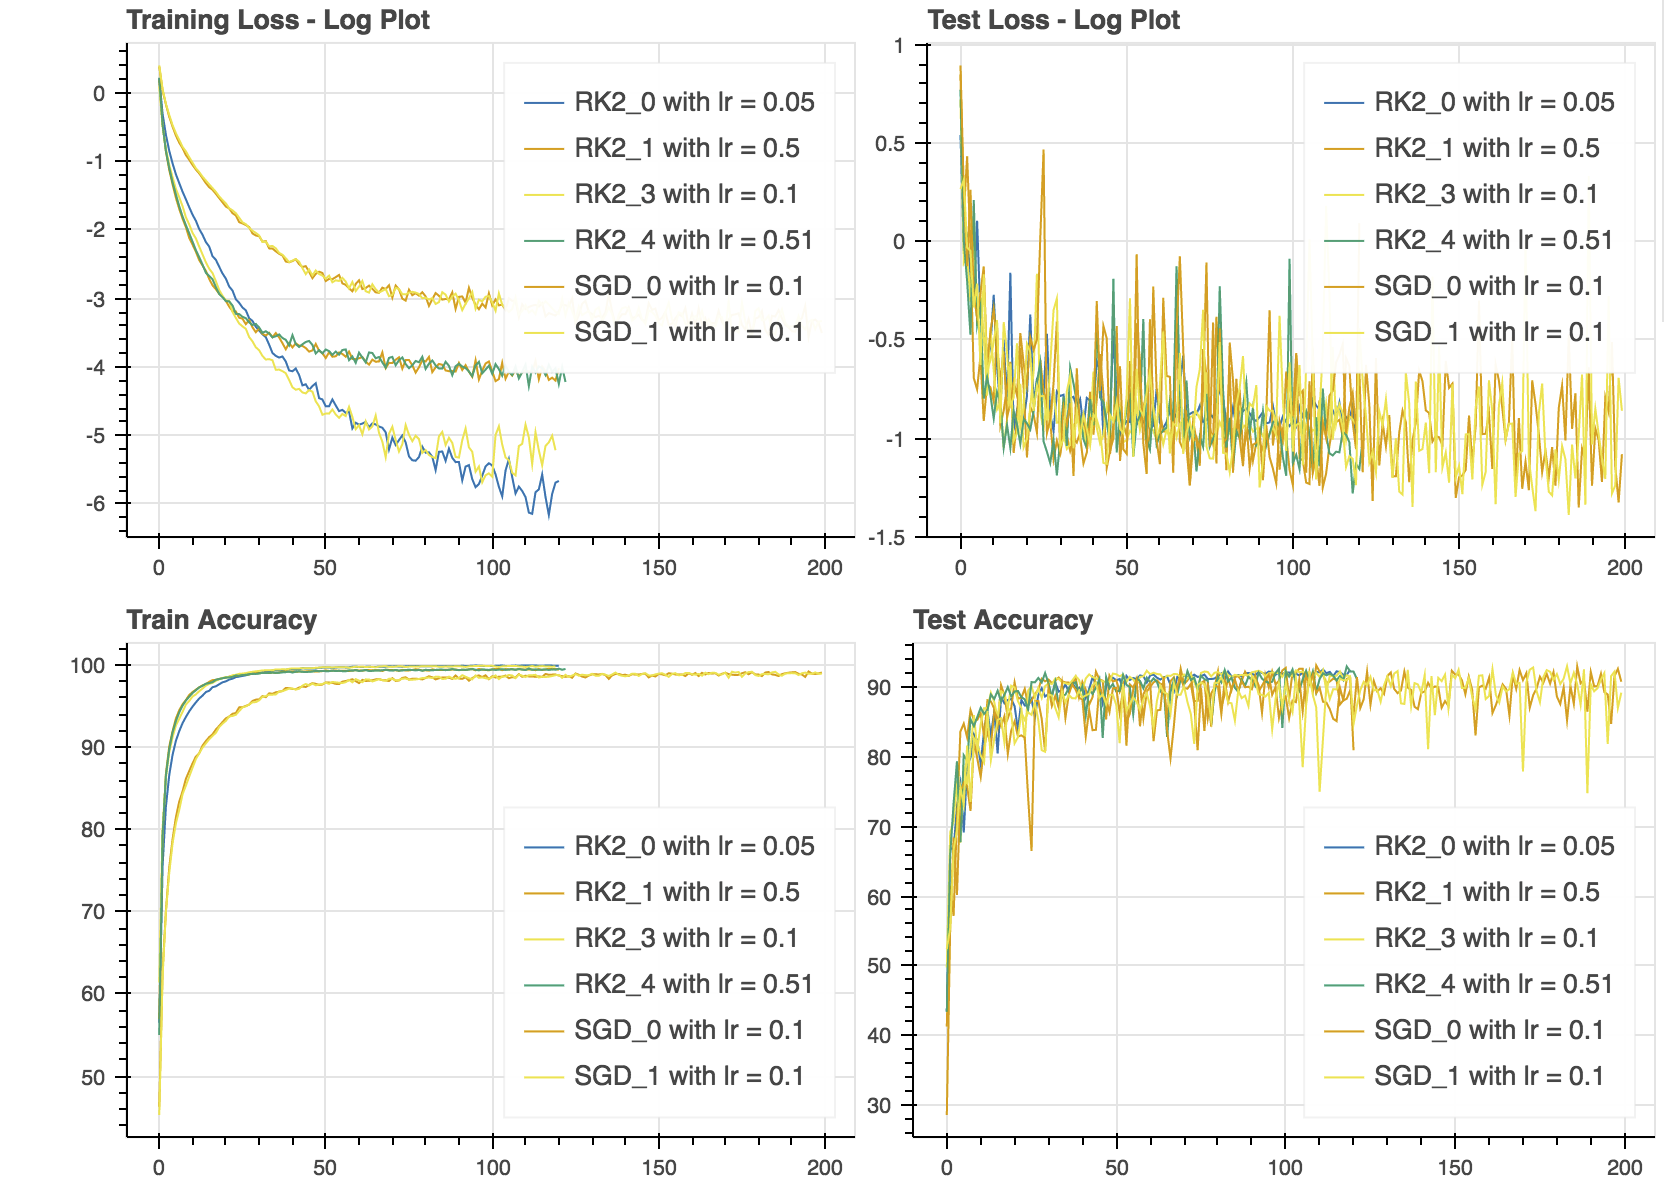
\includegraphics[width=0.8\linewidth]{../plots/inf_plots/wideresnet_rk2_sgd.png}
\end{center}\vspace{1cm}
\subsection*{Regression}
\begin{center}\vspace{1cm}
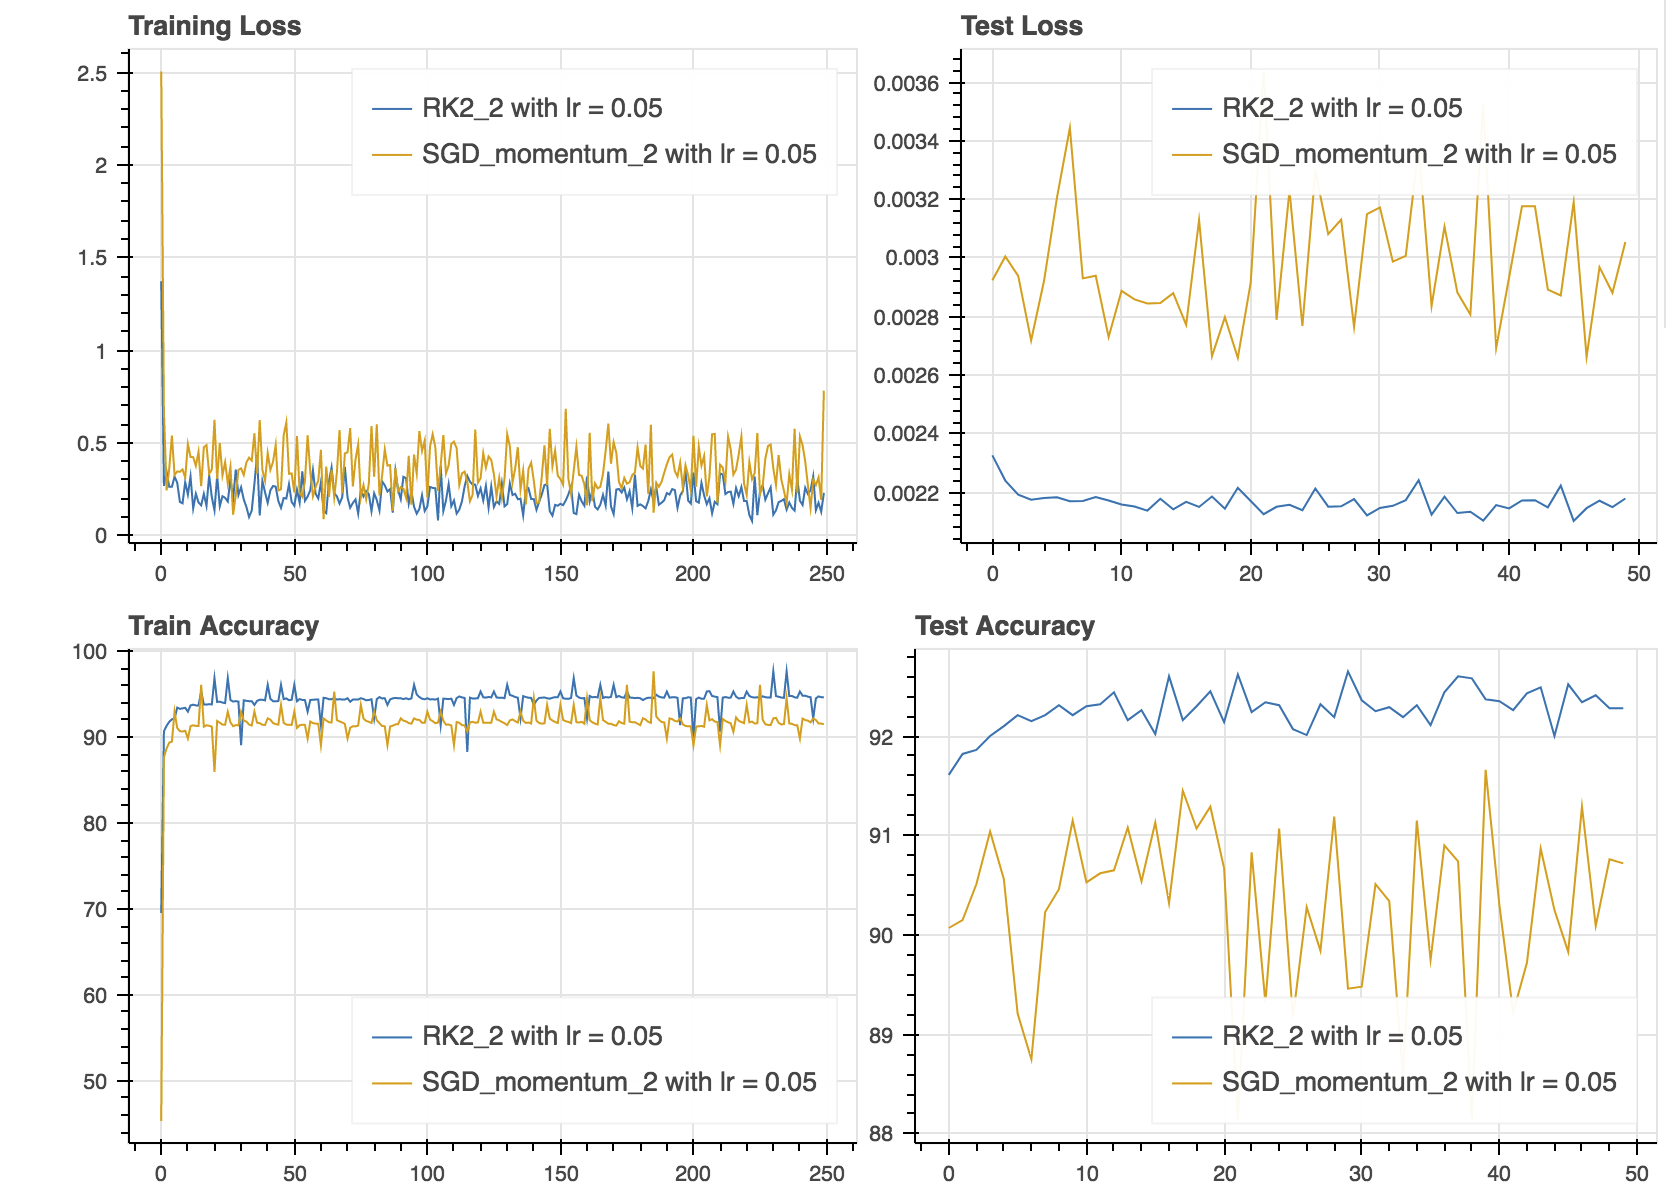
\includegraphics[width=0.8\linewidth]{../plots/plots_1/lasso_3.png}
\end{center}\vspace{1cm}

% \subsection*{Geothermal Conceptual Models}
% \begin{center}\vspace{1cm}
% \includegraphics[width=1.0\linewidth]{Algerian_geothermal_models.jpg}
% \captionof{figure}{\color{Green} (a) Idealized northern Algerian geothermal system characterized by heating of the filtered meteoric water. (b) Idealized southern Algerian geothermal system, characterized by basement heating of the sedimentary basin (Saibi, 2009)}
% \end{center}

%----------------------------------------------------------------------------------------
% CONCLUSIONS
%----------------------------------------------------------------------------------------

\color{Navy} % SaddleBrown color for the conclusions to make them stand out

\section*{Conclusions}
We aim to explore these methods further and see what concepts and methods from Numerical Analysis can shed light on the performance of Optimization Scheme, for instance stability, stiff equations, etc.
\color{Black} % Set the color back to DarkSlateGray for the rest of the content

 %----------------------------------------------------------------------------------------
% REFERENCES
%----------------------------------------------------------------------------------------

\nocite{*} % Print all references regardless of whether they were cited in the poster or not
\bibliographystyle{plain} % Plain referencing style
%!TEX root = main.tex
\begin{thebibliography}{9}
\bibitem{su}
 Su, Weijie, Stephen Boyd, and Emmanuel Candes. \textit{A differential equation for modeling Nesterov’s accelerated gradient method: Theory and insights}. Advances in Neural Information Processing Systems. 2014.

\bibitem{integration}
Scieur, Damien, et al. \textit{Integration Methods and Accelerated Optimization Algorithms} arXiv preprint arXiv:1702.06751 (2017).

\bibitem{nesterov}
Nesterov, Yurii. \textit{Introductory lectures on convex optimization: A basic course}. Vol. 87. Springer Science and Business Media, 2013.

\end{thebibliography}
 % Use the example bibliography file sample.bib

%----------------------------------------------------------------------------------------

\end{multicols}
\end{document}
